\chapter{Background}\label{ch:background}
\section{MicroHs}\label{sec:background:microhs}

MicroHs is a small Haskell compiler that has a relatively standard compilation pipeline. The compiler starts by parsing the Haskell source code into an abstract syntax tree (AST). The AST is then type-checked and subsequently desugared into lambda terms. The lambda terms are optimized and then transformed into combinators through the use of a process called bracket abstraction. After which the abstract representation of the combinators is converted into a useable format for the runtime written in C. When this is done, the runtime system and combinators are combined into a single C codebase, which is then either compiled to a native executable using a standard C compiler or converted to WebAssembly using Emscripten We are mostly interested in the final stages of the pipeline. The process is illustrated in Figure~\ref{fig:microhs-pipeline}. The compiler is bootstrapped, meaning that it is written in Haskell and compiles itself. The source code for the compiler can be found on GitHub~\cite{microhsrepo}.

\begin{figure}[t]
\centering
\resizebox{\textwidth}{!}{%
\begin{tikzpicture}[node distance=2cm]
\node (source) [textblock] {Haskell Source Code};
\node (lex) [process, right of=source, xshift=4cm] {Lexing and Parsing};
\node (typecheck) [process, right of=lex, xshift=4cm] {Type Checking};
\node (desugar) [process, below of=typecheck] {Desugaring};
\node (optimize) [process, below of=lex] {Optimization};
\node (bracket) [process, below of=source] {Bracket Abstraction};
\node (codegen) [process, below of=bracket] {Code Generation};
\node (runtime) [process, below of=optimize] {Runtime System Inclusion};
\node (target) [process, below of=runtime] {Target?};
\node (emscripten) [process, right of=target, xshift=4cm] {Call Emscripten};
\node (ccompiler) [process, left of=target, xshift=-4cm] {Call C Compiler};
\node (output1) [textblock, below of=ccompiler] {Native Executable};
\node (output2) [textblock, below of=emscripten] {WebAssembly Module};
\draw [arrow] (source) -- (lex);
\draw [arrow] (lex) -- node[anchor=south] {AST} (typecheck);
\draw [arrow] (typecheck) -- node[anchor=east] {AST} (desugar);
\draw [arrow] (desugar) -- node[anchor=south] {Lambda Terms} (optimize);
\draw [arrow] (optimize) -- node[anchor=south] {Lambda Terms} (bracket);
\draw [arrow] (bracket) -- node[anchor=east] {Combinators} (codegen);
\draw [arrow] (codegen) -- node[anchor=south] {C Code} (runtime);
\draw [arrow] (runtime) -- node[anchor=east] {C Code} (target);
\draw [arrow] (target) -- node[anchor=south] {Native} (ccompiler);
\draw [arrow] (target) -- node[anchor=south] {Wasm} (emscripten);
\draw [arrow] (ccompiler) -- (output1);
\draw [arrow] (emscripten) -- (output2);
\end{tikzpicture}
}
\caption{MicroHs Compilation Pipeline}
\label{fig:microhs-pipeline}
\end{figure}

\paragraph{Combinators}
MicroHs uses a combination of SKI combinators, an extended set of combinators, and primitive operations (intrinsics for arithmetic, I/O, etc.) to represent Haskell code. SKI combinators are a small set of combinators that can be used to represent any lambda term. The three basic SKI combinators are:
\begin{align*}
    S \; x \; y \; z & = x \; z \; (y \; z) \\
    K \; x \; y & = x \\
    I \; x & = x
\end{align*}
Further combinators include those used by Turner~\cite{turner} or are added by MicroHs itself to improve performance of the generated code. The reduction rules for these combinators are as follows:
\begin{align*}
    B \; x \; y \; z & = x \; (y \; z) \\
    C \; x \; y \; z & = x \; z \; y \\
    S' \; x \; y \; z \; w & = x \; (y \; w) \; (z \; w) \\
    B' \; x \; y \; z \; w & = x \; y \; (z \; w) \\
    C' \; x \; y \; z \; w & = x \; (y \; w) \; z \\
    A \; x \; y & = y \\
    U \; x \; y & = y \; x \\
    Z \; x \; y \; z & = x \; y \\
    P \; x \; y \; z & = z \; x \; y \\
    R \; x \; y \; z & = y \; z \; x \\
    O \; x \; y \; z \; w & = w \; x \; y \\
    Y \; x & = x \; (Y \; x) \\
    K2 \; x \; y \; z & = x \\
    K3 \; x \; y \; z \; w & = x \\
    K4 \; x \; y \; z \; w \; v & = x
\end{align*}

\paragraph{Representing Combinators}
To efficiently represent combinators and their arguments, MicroHs uses a graph representation. Each node can either be a leave node storing a combinator or a primitive value, or an internal node storing a reference to its left and right children. This allows for efficient sharing of subterms and avoids the need for copying when reducing combinators. For example, the combinator application \texttt{K (I x) y} can be represented as the graph shown in Figure~\ref{fig:combinator-graph}.
\begin{figure}[t]
\centering
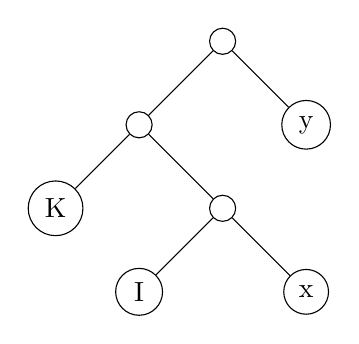
\begin{tikzpicture}[node distance=1.5cm]
\node (internal1) [circle, draw] {};
\node (internal2) [circle, draw, below left of=internal1] {};
\node (internal3) [circle, draw, below right of=internal2] {};
\node (k) [circle, draw, below left of=internal2] {K};
\node (i) [circle, draw, below left of=internal3] {I};
\node (x) [circle, draw, below right of=internal3] {x};
\node (y) [circle, draw, below right of=internal1] {y};
\draw (internal1) -- (internal2);
\draw (internal2) -- (internal3);
\draw (internal2) -- (k);
\draw (internal3) -- (i);
\draw (internal3) -- (x);
\draw (internal1) -- (y);
\end{tikzpicture}
\caption{Graph representation of the combinator application \texttt{K (I x) y}}
\label{fig:combinator-graph}
\end{figure}

\paragraph{Runtime System}
After building the graph representation of the combinators, the runtime system is responsible for reducing the graph to weak head normal form (WHNF). This is done by repeatadly walking the left spine of the graph until a leaf storing a combinator is reached, at which point the reduction rules for that combinator are applied. Since the reduction rules for most combinators involve multiple arguments, the runtime system maintains a left ancestor stack (LAS) to keep track of the ancestors of the current node (the left spine of the graph). This allows the runtime system to efficiently access the arguments needed for reduction without having to traverse the graph multiple times. An example reduction for the combinator application \texttt{K (I x) y} is shown in Figure~\ref{fig:combinator-reduction}. 

Another important thing to note about the runtime system is the existence of strict primitives, such as arithmetic operations, which require all of their arguments to be fully reduced before they can be applied. This means that when the runtime system encounters a strict primitive, it must first reduce all of its arguments to WHNF before applying the primitive operation and continuing with the reduction of the resulting graph.

\begin{figure}[t]
\centering
\begin{subfigure}[t]{0.45\textwidth}
\centering
\begin{tikzpicture}[node distance=1.5cm]
\node (internal1) [circle, draw] {};
\node (internal2) [circle, draw, below left of=internal1] {};
\node (y) [circle, draw, below right of=internal1] {y};
\draw (internal1) -- (internal2);
\draw (internal1) -- (y);
% current pointer
\node (cur) [rectangle, left of=internal1] {current};
\draw [arrow] (cur) -- (internal1);
\end{tikzpicture}
\caption{Start}
\end{subfigure}
\begin{subfigure}[t]{0.45\textwidth}
\centering
\begin{tikzpicture}[node distance=1.5cm]
\node (internal1) [circle, draw] {};
\node (internal2) [circle, draw, below left of=internal1] {};
\node (internal3) [circle, draw, below right of=internal2] {};
\node (y) [circle, draw, below right of=internal1] {y};
\node (k) [circle, draw, below left of=internal2] {K};
\draw (internal1) -- (internal2);
\draw (internal1) -- (y);
\draw (internal2) -- (internal3);
\draw (internal2) -- (k);
% current pointer
\node (cur) [rectangle, left of=internal2] {current};
\draw [arrow] (cur) -- (internal2);
% left ancestor stack
\node (las) [rectangle, anchor=south east] at (current bounding box.north west |- internal1) {LAS:};
\node (stack) [stack=1, anchor=west] at (las.east) {
  \nodepart{one} 
};
\draw [arrow] (stack.one) -- (internal1);
\end{tikzpicture}
\caption{Step left}
\end{subfigure}
\vfill
\begin{subfigure}[t]{0.45\textwidth}
\centering
\begin{tikzpicture}[node distance=1.5cm]
\node (internal1) [circle, draw] {};
\node (internal2) [circle, draw, below left of=internal1] {};
\node (internal3) [circle, draw, below right of=internal2] {};
\node (y) [circle, draw, below right of=internal1] {y};
\node (k) [circle, draw, below left of=internal2] {K};
\draw (internal1) -- (internal2);
\draw (internal1) -- (y);
\draw (internal2) -- (internal3);
\draw (internal2) -- (k);
% current pointer
\node (cur) [rectangle, left of=k] {current};
\draw [arrow] (cur) -- (k);
% left ancestor stack
\node (las) [rectangle, anchor=south east] at (current bounding box.north west |- internal1) {LAS:};
\node (stack) [stack=2, anchor=west, yshift=-0.2cm] at (las.east) {
  \nodepart{one} 
  \nodepart{two} 
};
\draw [arrow] (stack.one) -- (internal1);
\draw [arrow] (stack.two) -- (internal2);
\end{tikzpicture}
\caption{Step left}
\end{subfigure}
\begin{subfigure}[t]{0.45\textwidth}
\centering
\begin{tikzpicture}[node distance=1.5cm]
\node (internal1) [circle, draw] {};
\node (i) [circle, draw, below left of=internal1] {I};
\node (x) [circle, draw, below right of=internal1] {x};
\draw (internal1) -- (i);
\draw (internal1) -- (x);
% current pointer
\node (cur) [rectangle, left of=internal1] {current};
\draw [arrow] (cur) -- (internal1);
\end{tikzpicture}
\caption{Reduce K}
\end{subfigure}
\vfill
\begin{subfigure}[t]{0.45\textwidth}
\centering
\begin{tikzpicture}[node distance=1.5cm]
\node (internal1) [circle, draw] {};
\node (i) [circle, draw, below left of=internal1] {I};
\node (x) [circle, draw, below right of=internal1] {x};
\draw (internal1) -- (i);
\draw (internal1) -- (x);
% current pointer
\node (cur) [rectangle, left of=i] {current};
\draw [arrow] (cur) -- (i);
% left ancestor stack
\node (las) [rectangle, anchor=south east] at (current bounding box.north west |- internal1) {LAS:};
\node (stack) [stack=1, anchor=west] at (las.east) {
  \nodepart{one} 
};
\draw [arrow] (stack.one) -- (internal1);
\end{tikzpicture}
\caption{Step left}
\end{subfigure}
\begin{subfigure}[t]{0.45\textwidth}
\centering
\begin{tikzpicture}[node distance=1.5cm]
\node (x) [circle, draw] {x};
% current pointer
\node (cur) [rectangle, left of=x] {current};
\draw [arrow] (cur) -- (x);
\end{tikzpicture}
\caption{Reduce I}
\end{subfigure}
\caption{Reduction of the combinator application \texttt{K (I x) y}}
\label{fig:combinator-reduction}
\end{figure}

\section{WebAssembly}\label{sec:background:wasm}
Wasm is a binary stack-based instruction format. Wasm programs are ran inside a host environment that can influence the wasm code through imports and exports. The programs themselves are organized into modules containing functions, memory, imports/exports, and other components.

Wasm has a text format called WAT (WebAssembly Text format) which is a human-readable representation of the binary format. From now on we will use WAT syntax to illustrate Wasm concepts. Using WAT a simple list of instructions that adds two numbers looks like this:
\begin{minted}{wat}
(i32.const 1)
(i32.const 2)
(i32.add)
\end{minted}
The first two instructions push the constants 1 and 2 onto the stack, and the last instruction pops the two values from the stack, adds them together, and pushes the result (3) back onto the stack.

\paragraph{Instructions}
Instructions in Wasm are the basic building blocks of computation. They can be broadly categorized into two types: control flow instructions and simple instructions.

Simple instructions perform basic operations such as arithmetic, logical operations, and memory access. Examples include \texttt{i32.add} for adding two 32-bit integers, \texttt{i32.sub} for subtraction, and \texttt{local.get} and \texttt{local.set} for accessing local variables.

Control flow instructions manage the flow of execution within a function. Examples include \texttt{if}, \texttt{block}, \texttt{loop}, and \texttt{br} (branch). These instructions allow for conditional execution, loops, and jumps within the function body. Since Wasm does not have boolean types, conditions are represented using integers, where 0 is false and any non-zero value is true. When branching to a label belonging to a block, the execution continues after the end of the block. A loop label, on the other hand, causes execution to continue at the beginning of the loop. An example of the control flow instructions in action is shown below:
\begin{minted}{wat}
(block $exit
  (loop $loop
    ;; check if counter == 0
    (local.get $counter)
    (i32.const 0)
    (i32.eq)
    (br_if $exit) ;; if counter == 0, exit block
    ;; decrease counter
    (local.get $counter)
    (i32.const 1)
    (i32.sub)
    (local.set $counter)
    (br $loop) ;; continue looping
  )
)
\end{minted}

\paragraph{Functions}
Functions in Wasm consist of zero or more parameters, results, and local variables, and a body containing instructions. A simple function that adds two numbers and doubles the result can be defined like this:
\begin{minted}{wat}
(func $addAndDouble (param $a i32) (param $b i32) (result i32)
  (local $sum i32)
  (local.get $a)
  (local.get $b)
  (i32.add)
  (local.set $sum)
  (local.get $sum)
  (local.get $sum)
  (i32.add)
)
\end{minted}
In this example the function takes two parameters of type \texttt{i32} and returns a single \texttt{i32} result. The body of the function retrieves the parameters from the stack, adds them together, stores the result in a local variable, and then doubles the result by adding it to itself before returning it (a return is done by leaving the result on the stack at the end of the function body).

Functions can be called using the \texttt{call} instruction, which takes the function identifier as an argument and expects the appropriate number of arguments to be on the stack:
\begin{minted}{wat}
(i32.const 1)
(i32.const 2)
(call $add)
\end{minted}

\paragraph{Types}
Wasm has a couple of different categories of types, the most basic ones are the primitive numeric types, these include \texttt{i32} (32-bit integer), \texttt{i64} (64-bit integer), \texttt{f32} (32-bit float), and \texttt{f64} (64-bit float), as well as \texttt{v128} (128-bit SIMD vector). 

We can also box types through the use of references (note that references are explicitly typed in Wasm, meaning that every reference has a specific type associated with it), these have special instructions for manipulating them: \texttt{ref.null}, \texttt{ref.is\_null}, \texttt{ref.cast}, \texttt{ref.test}, and \texttt{ref.eq}. \texttt{ref.null} creates a null reference of a given type, \texttt{ref.is\_null} checks if a reference is null, \texttt{ref.cast} casts a reference to a different type (and traps if the cast is invalid), \texttt{ref.test} checks if a reference can be cast to a given type, and \texttt{ref.eq} compares two references.

These reference types can be used for boxing numeric types, but are most oftenly used for more complex types named aggregate types. Aggregate types include Structs and Arrays, and are user defined. Structs are collections of named fields, each with their own type, while Arrays are collections of elements of the same type. An example of type definitions for node which we could use for the implementation of the MicroHs runtime system is shown below:
\begin{minted}{wat}
(type $Node (struct
  (field $left  (mut anyref))
  (field $right (mut anyref))
))
\end{minted}
In this definition, we use the \texttt{anyref} type which is a supertype of all reference types in Wasm. This allows us to store references to any type of object in the \texttt{left} and \texttt{right} fields of the \texttt{Node} struct, but comes at the cost of having to perform runtime type casts when accessing these fields. The \texttt{mut} keyword indicates that the fields are mutable, meaning that their values can be changed after the struct is created. Simlarly we can define an array type like this:
\begin{minted}{wat}
(type $NodeArray (array (mut (ref null $Node))))
\end{minted}

\paragraph{Memory}
Originally Wasm provided only one type of memory, namely linear memory, which is a contiguous, byte-addressable array of memory that can be read and written to from Wasm code. Linear memory is managed manually by the program, meaning that the program is, for example, responsible for not overwriting memory that is still needed, and is thus prone to memory issues caused by human error.

Since the release of WasmGC, Wasm now also supports garbage-collected (GC) memory, it does this by leveraging the host environment's garbage collector reclaim and allocate memory on behalf of the Wasm program. Objects pointed to by references are automatically stored in GC memory.